%%
%% This is file `sample-sigconf-biblatex.tex',
%% generated with the docstrip utility.
%%
%% The original source files were:
%%
%% samples.dtx  (with options: `all,proceedings,sigconf-biblatex')
%% 
%% IMPORTANT NOTICE:
%% 
%% For the copyright see the source file.
%% 
%% Any modified versions of this file must be renamed
%% with new filenames distinct from sample-sigconf-biblatex.tex.
%% 
%% For distribution of the original source see the terms
%% for copying and modification in the file samples.dtx.
%% 
%% This generated file may be distributed as long as the
%% original source files, as listed above, are part of the
%% same distribution. (The sources need not necessarily be
%% in the same archive or directory.)
%%
%%
%% Commands for TeXCount
%TC:macro \cite [option:text,text]
%TC:macro \citep [option:text,text]
%TC:macro \citet [option:text,text]
%TC:envir table 0 1
%TC:envir table* 0 1
%TC:envir tabular [ignore] word
%TC:envir displaymath 0 word
%TC:envir math 0 word
%TC:envir comment 0 0
%%
%%
%% The first command in your LaTeX source must be the \documentclass
%% command.
%%
%% For submission and review of your manuscript please change the
%% command to \documentclass[manuscript, screen, review]{acmart}.
%%
%% When submitting camera ready or to TAPS, please change the command
%% to \documentclass[sigconf]{acmart} or whichever template is required
%% for your publication.
%%
%%
\documentclass[sigconf,natbib=false]{acmart}
\usepackage{graphicx}
\usepackage{multirow}
\usepackage{booktabs}
\usepackage{geometry}

%%
%% \BibTeX command to typeset BibTeX logo in the docs
\AtBeginDocument{%
  \providecommand\BibTeX{{%
    Bib\TeX}}}

%% Rights management information.  This information is sent to you
%% when you complete the rights form.  These commands have SAMPLE
%% values in them; it is your responsibility as an author to replace
%% the commands and values with those provided to you when you
%% complete the rights form.
\setcopyright{acmlicensed}
\copyrightyear{2024}
\acmYear{2024}
\acmDOI{10.1145/3630744.3659831}

%% These commands are for a PROCEEDINGS abstract or paper.
\acmConference[WebSci '24]{16th ACM Web Science Conference 2024}{May 21--24, 2024}{Stuttgart, Germany}
%%
%%  Uncomment \acmBooktitle if the title of the proceedings is different
%%  from ``Proceedings of ...''!
%%
%%\acmBooktitle{Woodstock '18: ACM Symposium on Neural Gaze Detection,
%%  June 03--05, 2018, Woodstock, NY}
\acmISBN{978-1-4503-XXXX-X/18/06}


%%
%% Submission ID.
%% Use this when submitting an article to a sponsored event. You'll
%% receive a unique submission ID from the organizers
%% of the event, and this ID should be used as the parameter to this command.
%%\acmSubmissionID{123-A56-BU3}

%%
%% For managing citations, it is recommended to use bibliography
%% files in BibTeX format.
%%
%% You can then either use BibTeX with the ACM-Reference-Format style,
%% or BibLaTeX with the acmnumeric or acmauthoryear sytles, that include
%% support for advanced citation of software artefact from the
%% biblatex-software package, also separately available on CTAN.
%%
%% Look at the sample-*-biblatex.tex files for templates showcasing
%% the biblatex styles.
%%


%%
%% The majority of ACM publications use numbered citations and
%% references, obtained by selecting the acmnumeric BibLaTeX style.
%% The acmauthoryear BibLaTeX style switches to the "author year" style.
%%
%% If you are preparing content for an event
%% sponsored by ACM SIGGRAPH, you must use the acmauthoryear style of
%% citations and references.
%%
%% Bibliography style
% \RequirePackage[
%   datamodel=acmdatamodel,
%   style=acmnumeric,
%   ]{biblatex}

%% Declare bibliography sources (one \addbibresource command per source)
% \addbibresource{sample-base.bib}

\usepackage[numbers]{natbib}

\bibliographystyle{ACM-Reference-Format}


%%
%% end of the preamble, start of the body of the document source.
\begin{document}

%%
%% The "title" command has an optional parameter,
%% allowing the author to define a "short title" to be used in page headers.
\title{Assessing the Predictive Power of Social Media Data-Fed Large Language Models on Voter Behavior}


%%
%% The "author" command and its associated commands are used to define
%% the authors and their affiliations.
%% Of note is the shared affiliation of the first two authors, and the
%% "authornote" and "authornotemark" commands
%% used to denote shared contribution to the research.
\author{Ehsan Barkhordar}
\email{ebarkhordar23@ku.edu.tr}
\affiliation{%
  \institution{Koç University}
  \city{Istanbul}
  \country{Turkey}
}

\author{Şükrü Atsizelti}
\email{satsizelti22@ku.edu.tr}
\affiliation{%
  \institution{Koç University}
  \city{Istanbul}
  \country{Turkey}
}

%%
%% By default, the full list of authors will be used in the page
%% headers. Often, this list is too long, and will overlap
%% other information printed in the page headers. This command allows
%% the author to define a more concise list
%% of authors' names for this purpose.
\renewcommand{\shortauthors}{Trovato et al.}

%%
%% The abstract is a short summary of the work to be presented in the
%% article.
\begin{abstract}
This article explores how large language models (LLMs) can reflect human preferences and exhibit biases based on the diversity and type of input data. Utilizing survey data linked with tweets, we compare the predictive performance and bias manifestations of LLMs under three different data inclusion strategies: (1) using only demographic information, (2) combining demographic information with tweets, and (3) exclusively using tweets. The study finds that prompts enriched with tweets notably improve the predictive accuracy of models compared to those relying solely on demographic data. More importantly, the inclusion of dynamic, user-generated content like tweets not only reduces the oversimplification of individual identities but also lessens inherent biases, leading to more accurate and representative simulations of voter behavior. These findings underscore the critical role of data variety in LLM-based simulations, suggesting that integrating richer, real-time data sources can effectively diminish biases and enhance the models' ability to simulate complex human characteristics.
\end{abstract}

%%
%% The code below is generated by the tool at http://dl.acm.org/ccs.cfm.
%% Please copy and paste the code instead of the example below.
%%
\begin{CCSXML}
<ccs2012>
   <concept>
       <concept_id>10010405.10010455.10010461</concept_id>
       <concept_desc>Applied computing~Sociology</concept_desc>
       <concept_significance>500</concept_significance>
       </concept>
   <concept>
       <concept_id>10010147.10010341.10010370</concept_id>
       <concept_desc>Computing methodologies~Simulation evaluation</concept_desc>
       <concept_significance>500</concept_significance>
       </concept>
 </ccs2012>
\end{CCSXML}


\ccsdesc[500]{Applied computing~Sociology}
\ccsdesc[500]{Computing methodologies~Simulation evaluation}

%%
%% Keywords. The author(s) should pick words that accurately describe
%% the work being presented. Separate the keywords with commas.
\keywords{large language models, social media, voter behavior, predictive analytics}

% \received{20 February 2007}
% \received[revised]{12 March 2009}
% \received[accepted]{5 June 2009}

%%
%% This command processes the author and affiliation and title
%% information and builds the first part of the formatted document.
\maketitle

\section{Introduction}
This study aims to assess the predictive accuracy and bias of Large Language Models (LLMs) when fed with social media data in forecasting voter behavior. It has been argued that biases in the training data of large language models reflect the real tendencies in society \cite{Argyle2023}; simulation studies have been conducted based on the capacity of large language models to reflect society \cite{Agnew2024}. In this field, existing surveys or experiments are replicated using large language models, and their compatibility with existing survey and experiment results is examined \cite{Agnew2024, Aher2023}.

Discussions on whether large language models can replace actual survey and experiment participants have also brought up objections regarding the capacities of LLMs. For example, Ollion et al. \cite{Ollion2024} have made warnings revolving around the replicability, privacy, and language bias issues, cautioning researchers about using it for research without considering those problems. One significant problem of these studies is the representativeness of the created silicon participants. In their meaningfully named article “large language models cannot replace human participants because they cannot portray identity groups”, Wang et al. \cite{Wang2024} argue that these LLM-based studies suffer from misportrayal, group flattening, and identity essentialization. They attribute these problems to the training data, where the group-related information generally comes from out-group remarks not from in-group and the loss function that 'rewards the most likely output' \cite{Wang2024}.

This disposition to essentialize identities may lead to a nonproductive line of research where identities are linked with unchanging or fixed characteristics, behaviors, or ideas. Adding self-produced information to the simulation process instead of just demographic information may enrich the results and solve some of the problems that arose due to the lack of information about the related simulated identities. Secondly, feeding the simulations with real-world information about the user may prevent or balance the essentializing tendency of large language models by providing unfixed stances and opinions. On top of that, adding user-generated information may be the cure to the problem of the source of group-related informations \cite{Wang2024}, that is since they are expressed by the user they may reflect the real tendencies of a population, instead of the prejudices towards them.

In this study, we utilized large language models (LLMs) to assess their predictive power on voter behavior by employing different types of data inputs. Specifically, we compared the following three data input strategies:

\begin{figure*}[ht]
    \centering
    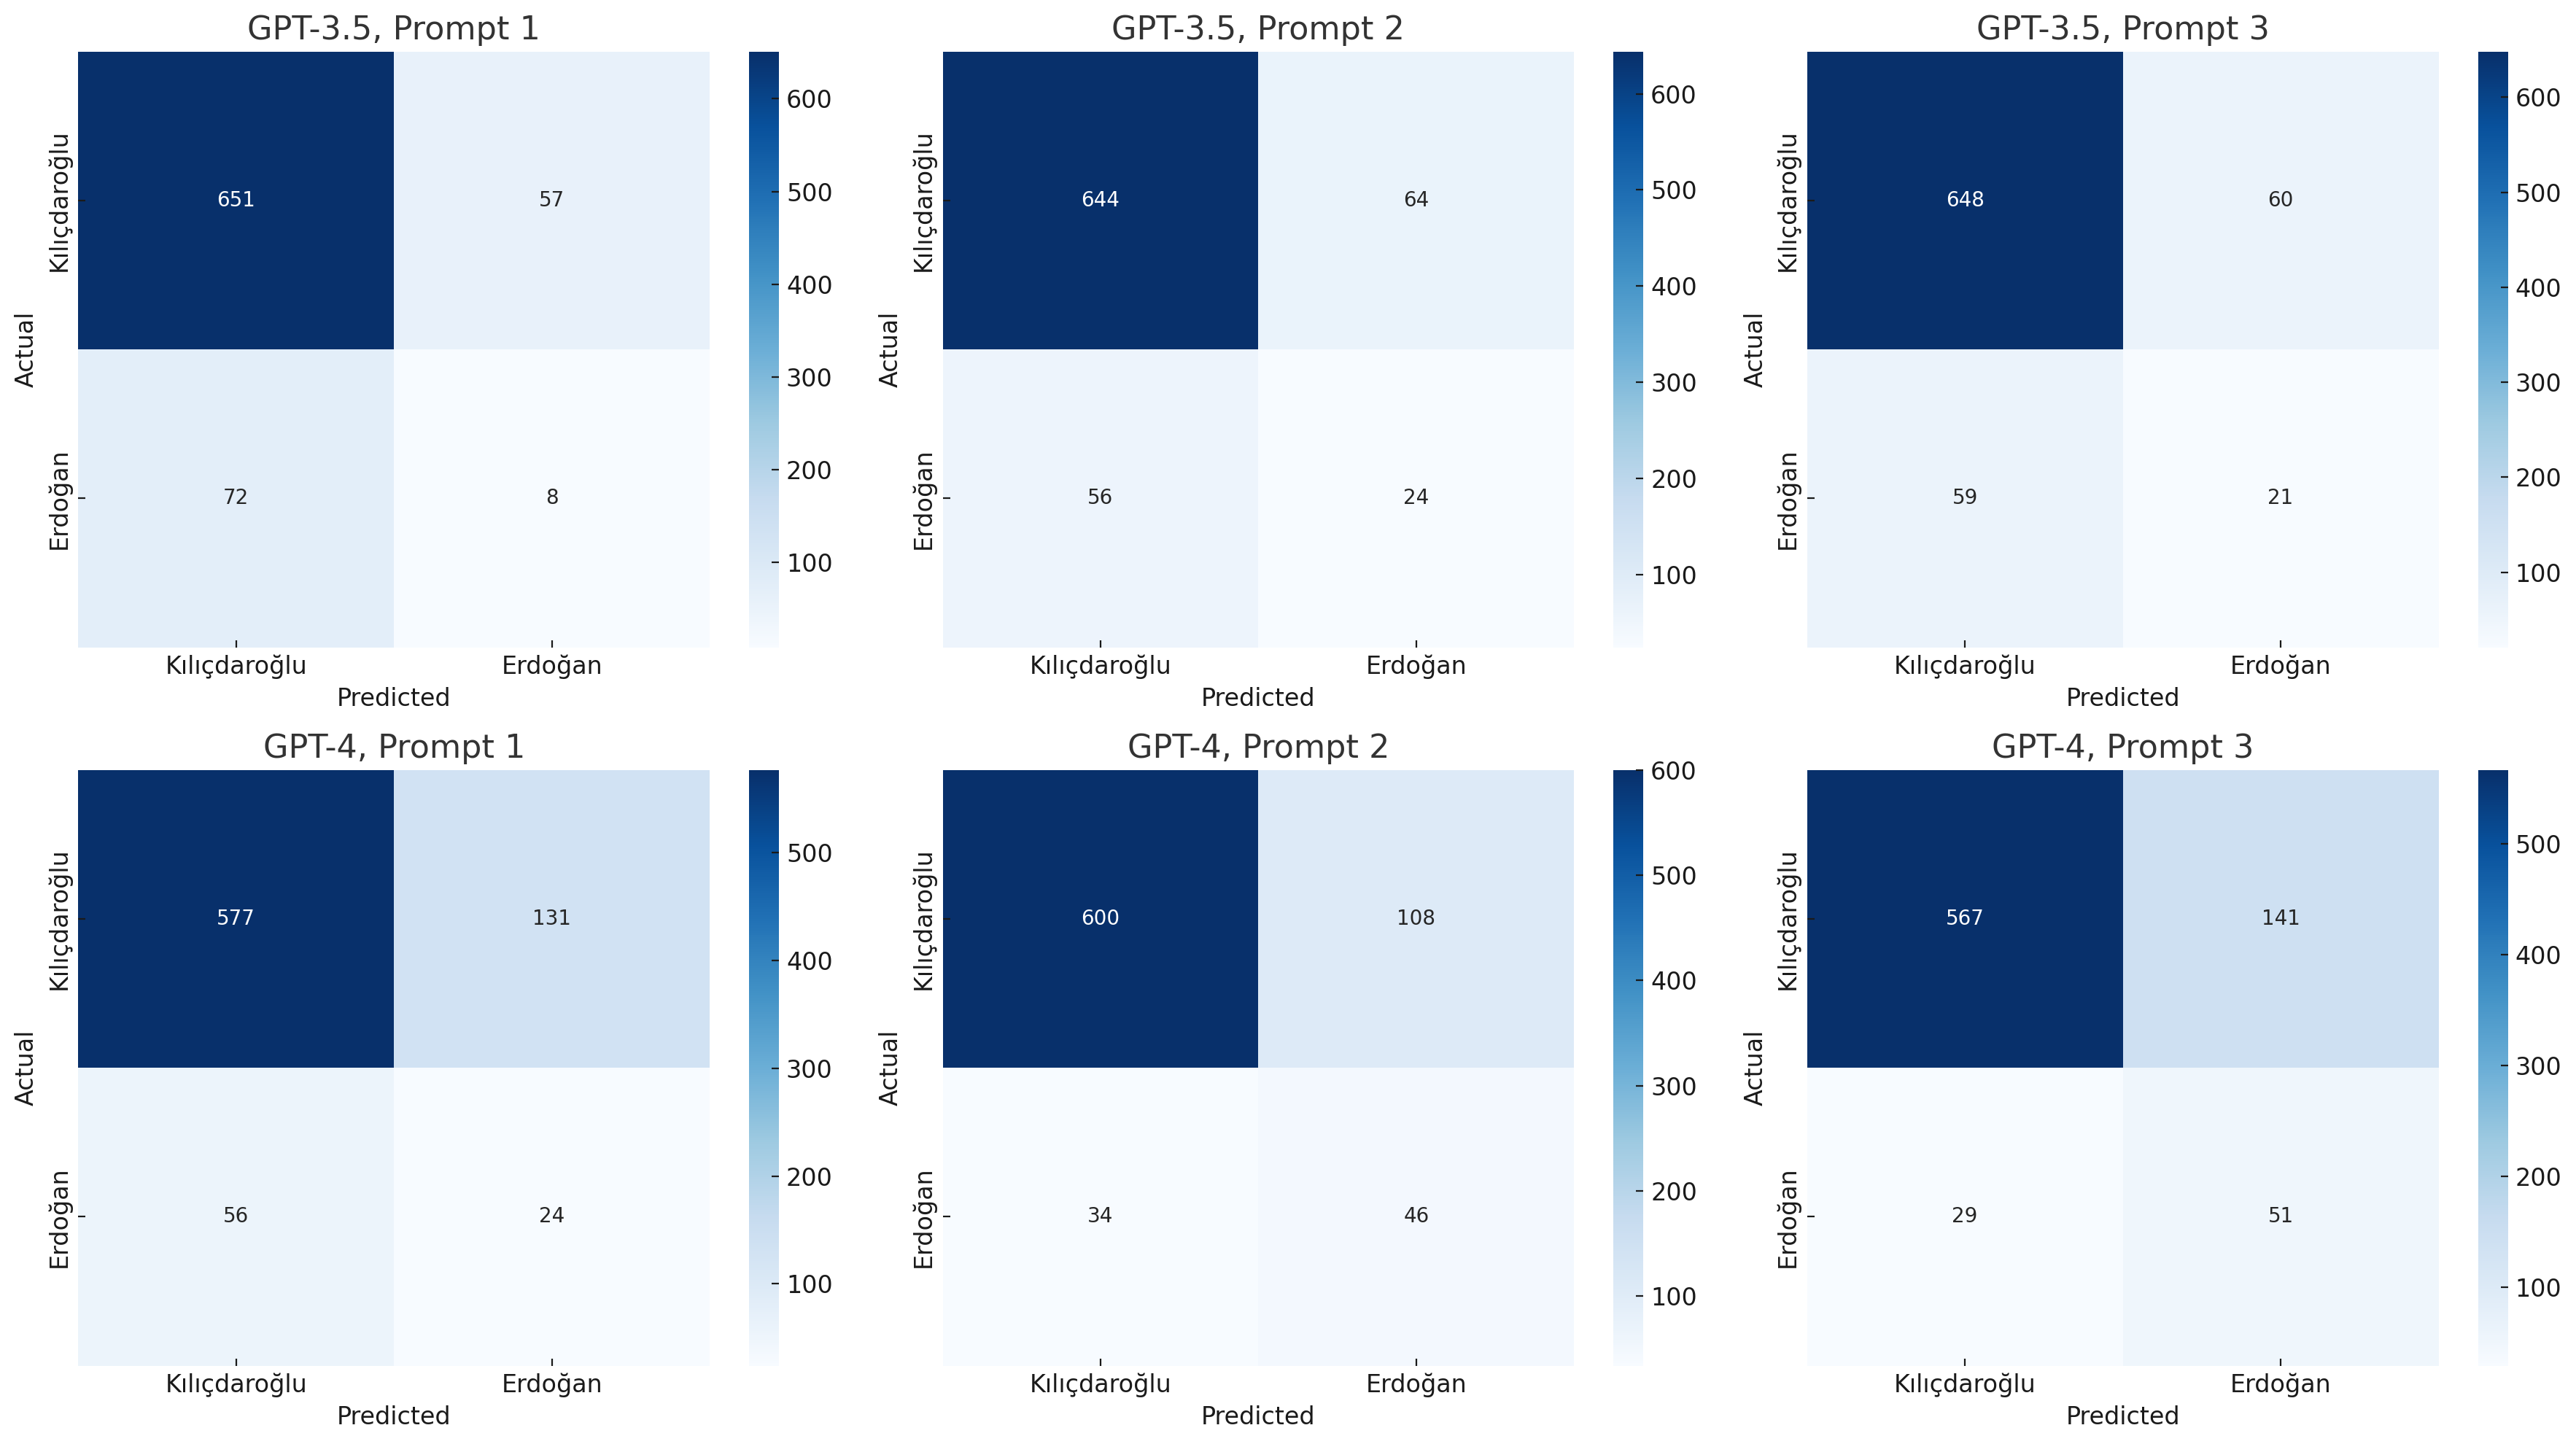
\includegraphics[width=\textwidth]{confusion_matrices.png}
    \caption{Confusion matrix of the different models and prompting strategies}
    \label{fig:confusion}
\end{figure*}

\begin{itemize}
    \item \textbf{Demographic Data Only:} The model was prompted using basic demographic information such as age, education, ethnicity, gender, and location.
    \item \textbf{Demographic Data with Tweets:} The model received a combination of demographic information and a random selection of 30 tweets, including favorites and retweets, from the user's Twitter account.
    \item \textbf{Tweets Only:} The model's input consisted solely of random tweets from the user's Twitter account.
\end{itemize}

The effectiveness of these scenarios was evaluated using precision, recall, and F1 scores for two versions of the models: GPT-3.5 \footnote{gpt-3.5-turbo-0125} and GPT-4-turbo \footnote{gpt-4-turbo-2024-04-09}. The results were then compared with the political preferences indicated by the users in a survey we conducted among Twitter users.

\section{Method}
This study is based on social media and survey data collected as part of the Politus project. The survey data was gathered between the first and second rounds of the 2023 Turkish presidential elections. The survey was conducted using Twitter ads and asked participants' consent to link their responses with their Twitter accounts, providing their usernames. Approximately 2,000 individuals completed the survey and half of these respondents' survey answers successfully linked with their Twitter accounts. Tweets from these linked profiles were then collected.

Prompts containing three different types of information were prepared and presented to two OpenAI models (GPT-3.5 and GPT-4-turbo). The first prompt included only demographic information (age, education, ethnicity, gender, and location) gathered from the survey. The second prompt included these demographic details plus a random selection of 30 tweets (including favorites and retweets) from the relevant user, while the third prompt contained only the random tweets. These prompts were used to predict which candidate the users likely voted for during the second round of the 2023 presidential elections. Responses indicating "I did not vote" in the survey were ignored in the analysis.


\subsection{Dataset}
The dataset comprises demographic data and linked Twitter data. Below are some examples from the demographic data:

\begin{table}[h]
  \caption{Examples from the demographic dataset}
  \label{tab:dataset}
  \begin{tabular}{ccccc}
    \toprule
    \textbf{Username} & \textbf{Age} & \textbf{Education} & \textbf{Ethnicity} & \textbf{City} \\
    \midrule
    user1 & 59 & university graduated & Turkish & Istanbul \\
    user2 & 37 & PhD holder & Turkish & Ankara \\
    user3 & 21 & high-school graduated & Turkish & Çanakkale \\
    user4 & 28 & master's degree & kurdish & Mardin \\
    user5 & 62 & university graduated & Arab & Adana \\
    \bottomrule
  \end{tabular}
\end{table}


    
\begin{table}[h]
  \caption{Political Support Distribution}
  \label{tab:supporters}
  \begin{tabular}{lcc}
    \toprule
    \textbf{Candidate} & \textbf{Number of Supporters} \\
    \midrule
    Kemal Kılıçdaroğlu & 708 \\
    Recep Tayyip Erdoğan & 80 \\
    \bottomrule
  \end{tabular}
\end{table}

\begin{figure}[ht]
  \centering
  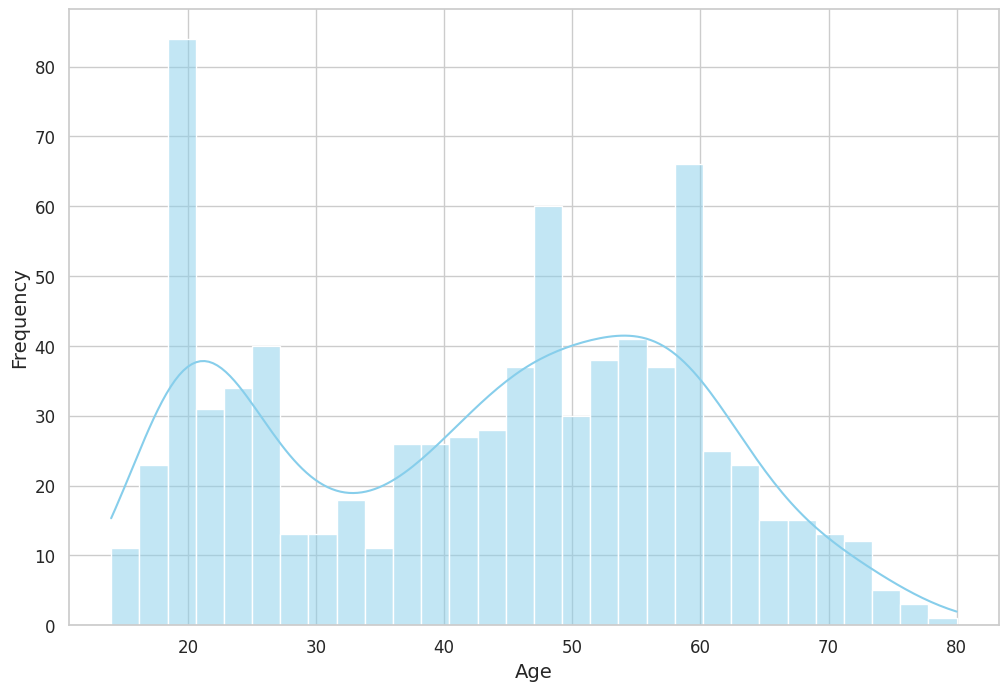
\includegraphics[width=\linewidth]{age.png}
  \caption{Age distribution of users in the dataset.}
  \label{fig:age_distribution}
\end{figure}


\begin{figure}[ht]
  \centering
  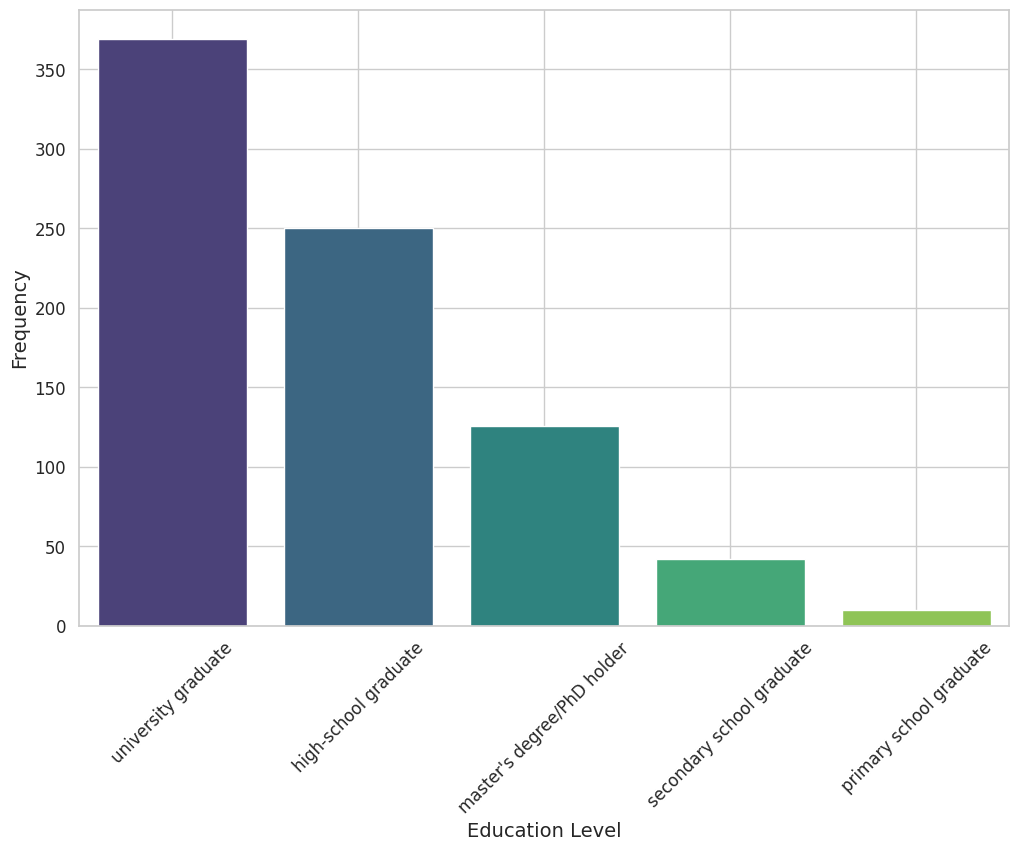
\includegraphics[width=\linewidth]{education.png}
  \caption{Education distribution of users in the dataset.}
  \label{fig:age_distribution}
\end{figure}


\section{Results and Discussions}
The general results indicate that the GPT-4-turbo model performed better than the GPT-3.5 model across all prompt types. Additionally, prompts that included social media data were more successful than those containing only demographic information. The most successful strategy, excluding the recall score of GPT-4-turbo, was when demographic information and tweets were presented together. Presenting only tweets was found to be more advantageous than presenting only demographic information.

\begin{figure}[ht]
  \centering
  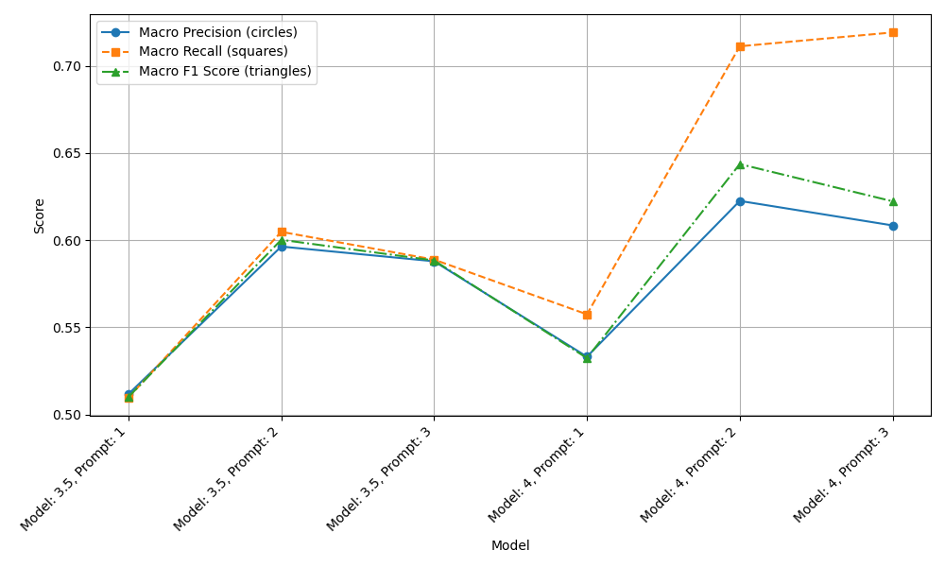
\includegraphics[width=\linewidth]{graph1.png}
  \caption{Performance scores of different models and prompting strategies.}
  \Description{This graph shows the performance scores for different models and prompting strategies, indicating that the combination of demographic data and tweets performs best.}
  \label{fig:graph1}
\end{figure}

Due to a significant imbalance between the two candidates' supporters among survey respondents, these numbers might be misleading. It is crucial to consider the supporters of each candidate separately to better assess the biases of different prompts and models. Figure \ref{fig:graph2} shows the precision, recall, and F1 scores for both groups separately. The scores for Kılıçdaroğlu supporters do not vary significantly across models, showing high precision, recall, and F1 scores. However, while Erdoğan supporters generally reflect the pattern observed in general scores, achieving the highest scores in the strategy combining demographic information with tweets (again, excluding the recall score of GPT-4-turbo), the scores for Kılıçdaroğlu supporters tend to decrease in the GPT-4-turbo model.

\begin{figure}[ht]
  \centering
  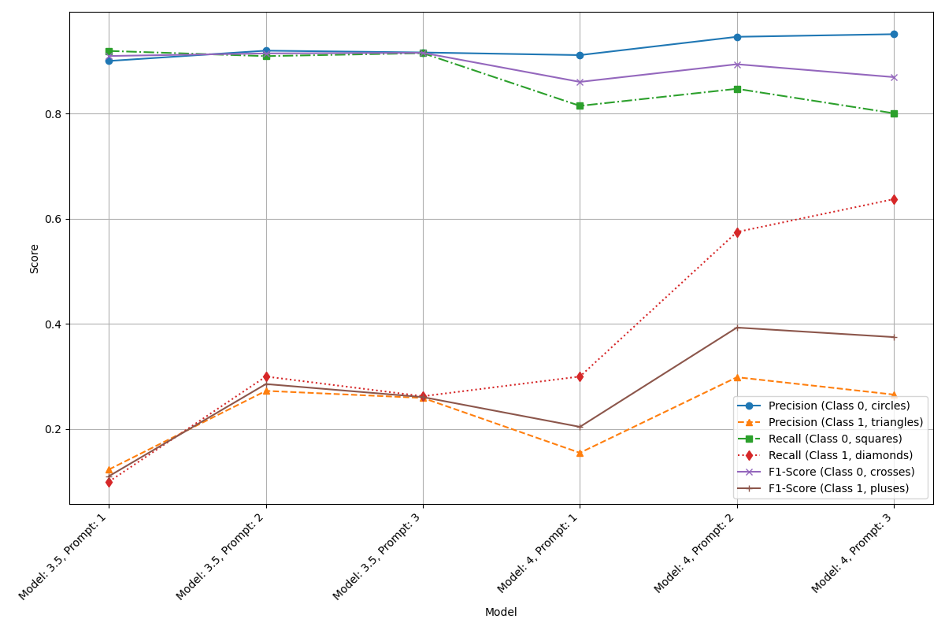
\includegraphics[width=\linewidth]{graph2.png}
  \caption{Performance scores for Kılıçdaroğlu and Erdoğan supporters.}
  \Description{This graph displays the performance scores for Kılıçdaroğlu and Erdoğan supporters separately, highlighting different trends in model accuracy between the two groups.}
   \label{fig:graph2}
\end{figure}

To address the imbalance issue, we analyzed a balanced sample of 180 respondents (80 Erdoğan supporters and 80 Kılıçdaroğlu supporters). The results are shown in Figure \ref{fig:graph3}. The balanced dataset analysis indicates that the overall trends remain consistent, with the GPT-4-turbo model outperforming across all prompting strategies. However, precision, recall, and F1 scores for both groups are more comparable, offering a clearer view of model performance without sample size imbalance.

\begin{figure}[ht]
  \centering
  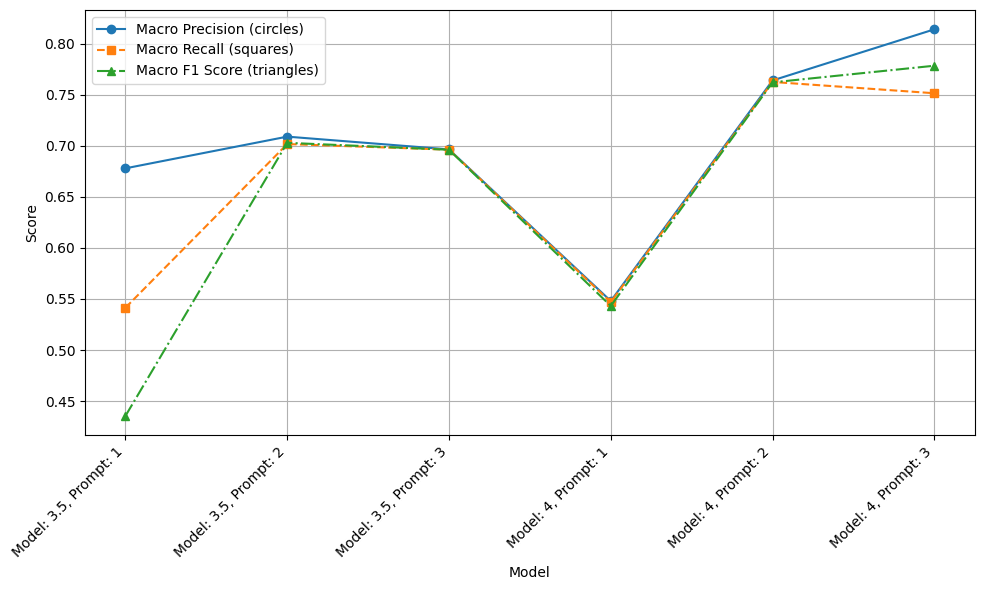
\includegraphics[width=\linewidth]{graph3.png}
  \caption{Performance scores of different models and prompting strategies with a balanced sample size (80 Erdoğan, 80 Kılıçdaroğlu).}
  \Description{This graph shows the performance scores for different models and prompting strategies with a balanced sample size, indicating consistent trends with the unbalanced analysis.}
  \label{fig:graph3}
\end{figure}

For Erdoğan supporters, models often misclassify them. The inclusion of tweets has enhanced model performance across all metrics. One might expect better identification of Erdoğan supporters when only tweets are used, as demographic information can be misleading. However, the highest recall scores were achieved with the GPT-4-turbo model using tweets without demographic data, while GPT-3.5 performance declined in this scenario.


\begin{figure}[ht]
  \centering
  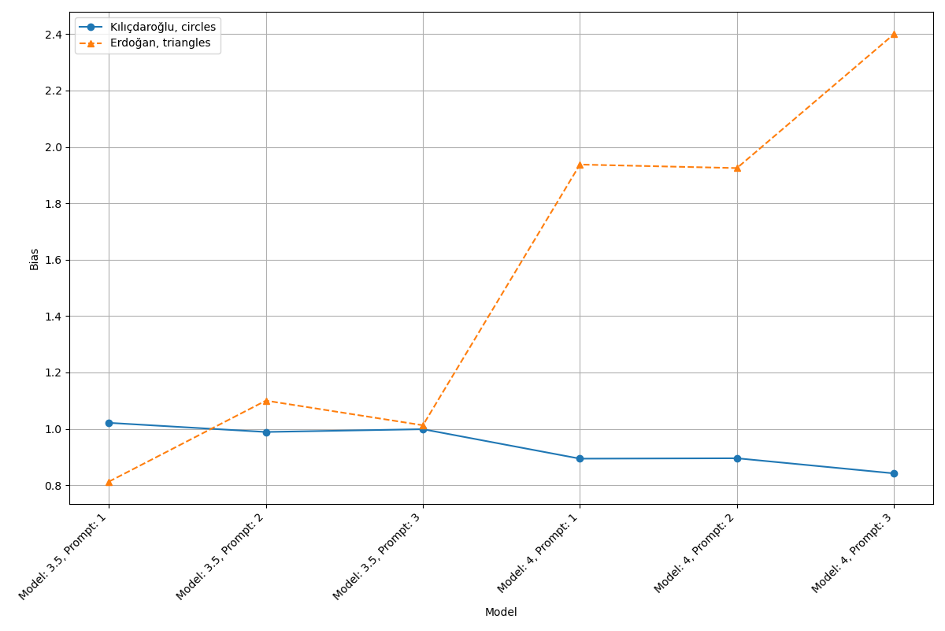
\includegraphics[width=\linewidth]{graph4.png}
  \caption{Class-specific bias comparison by model.}
  \Description{This graph shows a class-specific bias comparison by model, with a decrease in bias towards labeling users as Kılıçdaroğlu and an increase in labeling as Erdoğan in model 4 compared to model 3.5.}
\end{figure}

According to Figure \ref{fig:confusion}, models mark actual Erdoğan supporters as Kılıçdaroğlu supporters less frequently as we move from GPT-3.5 to GPT-4-turbo, and from prompts without tweets to those with tweets. Additionally, the tendency of models to misclassify Kılıçdaroğlu supporters as Erdoğan supporters has similarly increased. Beyond the differences between models, the inclusion of tweets also seems to have led models to better identify and overpredict Erdoğan. Examining results on individual levels can provide important insights about biases in the models. Unfortunately, data insufficiency makes it impossible to examine each level individually.


\section{Conclusion}
This study provided a comparative analysis of Large Language Models (LLMs) in terms of their ability to predict voter behavior using different types of data inputs, specifically demographic information versus social media content. Our findings demonstrate that LLMs incorporating a mix of demographic and tweet data deliver the most accurate predictions. This superior performance suggests that the integration of real-time, self-generated user data can significantly enhance the model's understanding of complex human behaviors and preferences, reducing the occurrence of biases typically seen in models trained solely on demographic data.

Moreover, the results highlight the importance of model version updates, as GPT-4-turbo outperformed its predecessor in all scenarios. This underscores the continuous improvements in model architectures and training methodologies, contributing to more sophisticated data processing capabilities.

\subsection{Limitations}
This study has several limitations. The dataset, primarily consisting of Twitter users, may not be fully representative of the general population, introducing a potential bias toward more tech-savvy individuals. Additionally, the imbalance in the number of supporters for each candidate could have influenced the model's performance. The focus on Twitter data alone may not capture the full spectrum of an individual's online behavior and preferences.

\subsection{Future Work}
Future research should expand datasets to include more diverse demographic groups and social media interactions. Exploring other social media platforms like Facebook, Instagram, and LinkedIn, as well as incorporating multi-modal data sources such as images and videos, could provide further insights. Investigating different data preprocessing techniques and model fine-tuning strategies could optimize performance. Longitudinal studies tracking voter behavior over time with continuous data collection methods could offer deeper insights into voter preference dynamics.



%%
%% Print the bibliography
%%
% \printbibliography
\bibliography{sample-base}


%%
%% If your work has an appendix, this is the place to put it.
\appendix


\end{document}
\endinput
%%
%% End of file `sample-sigconf-biblatex.tex'.
